% Options for packages loaded elsewhere
\PassOptionsToPackage{unicode}{hyperref}
\PassOptionsToPackage{hyphens}{url}
%
\documentclass[
]{book}
\usepackage{lmodern}
\usepackage{amssymb,amsmath}
\usepackage{ifxetex,ifluatex}
\ifnum 0\ifxetex 1\fi\ifluatex 1\fi=0 % if pdftex
  \usepackage[T1]{fontenc}
  \usepackage[utf8]{inputenc}
  \usepackage{textcomp} % provide euro and other symbols
\else % if luatex or xetex
  \usepackage{unicode-math}
  \defaultfontfeatures{Scale=MatchLowercase}
  \defaultfontfeatures[\rmfamily]{Ligatures=TeX,Scale=1}
\fi
% Use upquote if available, for straight quotes in verbatim environments
\IfFileExists{upquote.sty}{\usepackage{upquote}}{}
\IfFileExists{microtype.sty}{% use microtype if available
  \usepackage[]{microtype}
  \UseMicrotypeSet[protrusion]{basicmath} % disable protrusion for tt fonts
}{}
\makeatletter
\@ifundefined{KOMAClassName}{% if non-KOMA class
  \IfFileExists{parskip.sty}{%
    \usepackage{parskip}
  }{% else
    \setlength{\parindent}{0pt}
    \setlength{\parskip}{6pt plus 2pt minus 1pt}}
}{% if KOMA class
  \KOMAoptions{parskip=half}}
\makeatother
\usepackage{xcolor}
\IfFileExists{xurl.sty}{\usepackage{xurl}}{} % add URL line breaks if available
\IfFileExists{bookmark.sty}{\usepackage{bookmark}}{\usepackage{hyperref}}
\hypersetup{
  pdftitle={Matemáticas Financieras},
  pdfauthor={Eduardo Selim Martinez Mayorga},
  hidelinks,
  pdfcreator={LaTeX via pandoc}}
\urlstyle{same} % disable monospaced font for URLs
\usepackage{longtable,booktabs}
% Correct order of tables after \paragraph or \subparagraph
\usepackage{etoolbox}
\makeatletter
\patchcmd\longtable{\par}{\if@noskipsec\mbox{}\fi\par}{}{}
\makeatother
% Allow footnotes in longtable head/foot
\IfFileExists{footnotehyper.sty}{\usepackage{footnotehyper}}{\usepackage{footnote}}
\makesavenoteenv{longtable}
\usepackage{graphicx,grffile}
\makeatletter
\def\maxwidth{\ifdim\Gin@nat@width>\linewidth\linewidth\else\Gin@nat@width\fi}
\def\maxheight{\ifdim\Gin@nat@height>\textheight\textheight\else\Gin@nat@height\fi}
\makeatother
% Scale images if necessary, so that they will not overflow the page
% margins by default, and it is still possible to overwrite the defaults
% using explicit options in \includegraphics[width, height, ...]{}
\setkeys{Gin}{width=\maxwidth,height=\maxheight,keepaspectratio}
% Set default figure placement to htbp
\makeatletter
\def\fps@figure{htbp}
\makeatother
\setlength{\emergencystretch}{3em} % prevent overfull lines
\providecommand{\tightlist}{%
  \setlength{\itemsep}{0pt}\setlength{\parskip}{0pt}}
\setcounter{secnumdepth}{5}
\usepackage{booktabs}
\usepackage[]{natbib}
\bibliographystyle{plainnat}

\title{Matemáticas Financieras}
\author{Eduardo Selim Martinez Mayorga}
\date{2022-03-01}

\usepackage{amsthm}
\newtheorem{theorem}{Teorema}[chapter]
\newtheorem{lemma}{Lema}[chapter]
\newtheorem{corollary}{Corolario}[chapter]
\newtheorem{proposition}{Proposición}[chapter]
\newtheorem{conjecture}{Conjetura}[chapter]
\theoremstyle{definition}
\newtheorem{definition}{Definición}[chapter]
\theoremstyle{definition}
\newtheorem{example}{Ejemplo}[chapter]
\theoremstyle{definition}
\newtheorem{exercise}{Ejercicio}[chapter]
\theoremstyle{definition}
\newtheorem{hypothesis}{Hipotesis}[chapter]
\theoremstyle{remark}
\newtheorem*{remark}{Observación }
\newtheorem*{solution}{Solución }
\begin{document}
\maketitle

{
\setcounter{tocdepth}{1}
\tableofcontents
}
\hypertarget{teoruxeda-del-interuxe9s}{%
\chapter{Teoría del interés}\label{teoruxeda-del-interuxe9s}}

\begin{definition}[Definición de Interés]
El interés se puede definir como una compensación/beneficio que una parte A le da a una parte B por dejar de satisfacer una necesidad para que el otro satisfaga la propia.
\end{definition}

Solo pensando en términos monetarios\ldots{} ¿Por qué las inversiones (en teoría ) crecen?
Algunos factores que intervienen en una inversión:

\begin{itemize}
\tightlist
\item
  Dinero (¿cuánto tiempo?)
\item
  ¿En qué se invierte?
\item
  ¿Cuánto tiempo lo invierto?
\item
  Inflación
\item
  Bajo que condiciones contractuales lo invierto (¿cómo crece el dinero ?)
\item
  Oferta y demanda
\item
  ¿Cuándo lo invierto?
\end{itemize}

Por un momento(grande) pensemos que el nivel de inversión depende solo del tiempo.

\begin{theorem}
Se dice que una función \(a:\left[ 0,\infty \right) \longrightarrow \mathbb{R}\) es una función de acumulación si cumple:

\begin{enumerate}
\def\labelenumi{\arabic{enumi}.}
\tightlist
\item
  \(a(0) = 1\)
\item
  \(a\left(\cdot\right)\) es no-decreciente
\item
  \(a(\cdot)\) es continua por la derecha y con límite por la izquierda.
\end{enumerate}

\(a(t)\) representa el valor acumulado de \(\$1\) que hay durante un lapso de tiempo t.
\end{theorem}

\begin{example}

.

\begin{enumerate}
\def\labelenumi{\arabic{enumi}.}
\item
  \(a(t) = 1+ct\), \(c>0\), \(c\) constante (interés simple)
\item
  \(a(t) = e^{\alpha t}\), \(\alpha > 0\) (interés compuesto)
\item
  \(a(t) = ct^2 + 1\), \(c>0\)
\item
  \(a(t) = 1\)
\item
  \(a(t) = (1+t)^c\), \$c\textgreater0
\item
  \(a(t) = 1 + arctang(t)\)
\item
  \(a(t) = \sqrt{t+1}\)
\item
  \(a(t) = \sqrt{t} + 1\)
\item
  \(a(t) = 1 + c\left[ t \right]\)
\item
  \(a(t) = e^{\left[ t \right]}\)
\end{enumerate}

\end{example}

\begin{definition}
Se define la \textbf{función de monto} correspondiente a \(a(t)\) como un capital inicial \(k>0\), como
\[ A_k \left( t \right) : = k \cdot a \left( t\right)\]
\end{definition}

\begin{remark}
Se cumple (1) y (3), pero \(A_k(0) = k \cdot a(0) = k \cdot 1 = k\)
\end{remark}

\(A_k(t)\) representa el valor acumulado de una inversión de un lapso de tiempo t.

\textbf{Representación gráfica}

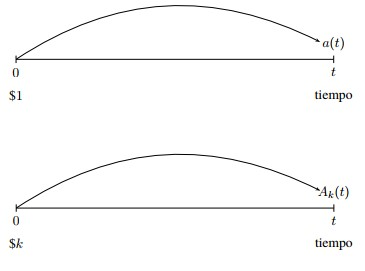
\includegraphics{images/1.jpg}

¿Cómo medimos el performance de una función de acumulación o función de monto?

Estudiaremos 3 indicadores:

\begin{enumerate}
\def\labelenumi{\arabic{enumi}.}
\tightlist
\item
  Tasa efectiva de interés al tiempo t
\item
  Tasa de descuento al tiempo t
\item
  Fuerza de interés
\end{enumerate}

\begin{definition}
Para una función de acumulación \(a\left( \cdot \right)\) se define la tasa efectiva de \underline{\textbf{interés al tiempo t}} como:
\[ i_t := \frac{a\left( t \right) - a\left( t -1 \right)}{a\left( t - 1 \right)}\]
\end{definition}

\textbf{Interpretación:} Por cada peso invertida al tiempo \(t-1\) hay \(i_t\) unidades de ganancia. ``Lo que yo gané por cada peso que invertí''.

\begin{example}

.

\begin{enumerate}
\def\labelenumi{\arabic{enumi}.}
\item
  Para \(a(t) = 1 + ct\)
  \(i_t = \frac{a\left( t \right) - a\left( t -1 \right)}{a\left( t - 1 \right)} = \frac{1 + ct - \left[ 1 + c(t-1)\right] }{1+c(t-1)} = \frac{c}{1+c(t-1)}\)
  Obsérvese que la aplicación \(t \longmapsto i_t = \frac{c}{1+c(t-1)}\) es \textbf{decreciente}.
  Con la función \(a(t) = 1 + ct\) ganamos, pero cada vez menos conforme el tiempo avanza.
\item
  Para \(a(t) = e^{\alpha t}\), \(\alpha > 0\)
  \(i_t = \frac{a\left( t \right) - a\left( t -1 \right)}{a\left( t - 1 \right)} = \frac{e^{\alpha t} - e^{\alpha (t-1)}}{e^{\alpha (t-1)}} = \frac{e^{\alpha (t-1)}\left[ e^{\alpha}-1\right]}{e^{\alpha (t-1)}} = e^{\alpha} -1\)
  Obsérvese que la aplicación \(t \longmapsto i_t = e^{\alpha} -1\) es \textbf{constante}.
\end{enumerate}

{tarea}

Para \(a(t)= e^{t^2}\) calcular \(i_t\) y ver si \(t \longmapsto i_t\) es creciente o decreciente

\begin{enumerate}
\def\labelenumi{\arabic{enumi}.}
\setcounter{enumi}{2}
\tightlist
\item
  \(a(t) = (1+c)^t\), \(c > 0\)
  \(i_t = \frac{a\left( t \right) - a\left( t -1 \right)}{a\left( t - 1 \right)} = \frac{(1+c)^t - (1+c)^{t-1}}{(1+c)^{t-1}} = \frac{(1+c)^{t-1}[(1+c)-1]}{(1+c)^{t-1}} = 1+c-1 = c\)
  Obsérvese que la aplicación \(t \longmapsto i_t = e^{\alpha} -1\) es \textbf{constante}.
\end{enumerate}

\end{example}

\begin{remark}
Los ejemplos 2 y 3 son los mismos
\((1+c)^t=e^{log\left((1+c)^t \right)} = e^{tlog(1+c)}=e^{\alpha t}\), con \(\alpha = log(1+c)\).

En el mundo financiero preferimos escribir a la función exponencial como \((1+c)^t\).
\end{remark}

\textbf{{Notación}}

En realidad preferimos escribir a la función exponencial como \(a(t) = (1+i)^t\). Bajo esta notación \(i_t = c = i\), es decir, \(i_t=i\).

Al número ``\(i\)'' le llamamos {tasa efectiva de interés}, y al modelo \(a(t)=(1+i)^t\) se le conoce como el {modelo de interés compuesto.}.

\begin{remark}
\(\frac{A_k(t)-A_k(t-1)}{A_k(t-1)}=\frac{ka(t) - ka(t-1)}{ka(t-1)} = \frac{a(t)-a(t-1)}{a(t-1)} = i_t\)
\end{remark}

\begin{definition}
Para una función de acumulación \(a(t)\) diferenciable, se define la \underline{\textcolor{blue}{fuerza de interés}} correspondiente a \(a(\cdot)\) como
\end{definition}

\begin{equation*}
\boxed{
\delta_t : = \frac{\frac{\partial}{\partial t} a(t)}{a(t)}
}\end{equation*}

¿De dónde viene esa definición?

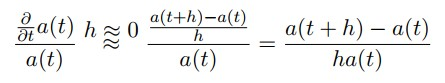
\includegraphics{images/2.jpg}

\begin{remark}
\(\delta_t\) también se puede obtener como \(\frac{\partial}{\partial t} log(a(t)) = \frac{a'(t)}{a(t)} = \delta_t\)
\end{remark}

\begin{example}
.

\begin{enumerate}
\def\labelenumi{\arabic{enumi}.}
\tightlist
\item
  \(a(t)=e^{\alpha t}\)
\end{enumerate}

\(\delta_t = \frac{a'(t)}{a(t)} = \frac{\left( e^{\alpha t}\right)'}{e^{\alpha t}} = \frac{\alpha e^{\alpha t}}{e^{\alpha t}} = \alpha\)

\(\therefore \delta_t = \alpha\), con \(\alpha\) constante

\begin{enumerate}
\def\labelenumi{\arabic{enumi}.}
\setcounter{enumi}{1}
\tightlist
\item
  \(a(t) = 1+ct\)
\end{enumerate}

\(\delta_t = \frac{a'(t)}{a(t)} = \frac{\left( 1+ct\right)'}{1+ct} = \frac{c}{1+ct}\)

\(\therefore t\longmapsto \delta_t\) es decreciente
\end{example}

\begin{definition}
Para una función de acumulación \(a(\cdot )\) se define la {tasa efectiva de descuento al tiempo t} como:
\begin{equation*}
\boxed{d_t := \frac{a(t)-a(t-1)}{a(t)}}
\end{equation*}
\end{definition}

También se conoce como tasa efectiva de descuento en el intervalo \(\left[ t-1, t\right]\). ¿Cómo se interpreta \(d_t\)?

Por cada unidad de \(a(t)\) hay \(d_t\) unidades de \(a(t)-a(t-1)\). ``Por cada peso obtenido hay \(d_t\) pesos de ganancia obtenida''.

\begin{example}
.

\begin{enumerate}
\def\labelenumi{\arabic{enumi}.}
\tightlist
\item
  \(a(t) = (1+i)^t\)
\end{enumerate}

\(d_t = \frac{a(t) - a(t-1)}{a(t)} = \frac{(1+i)^t - (1+i)^{t-1}}{(1+i)^t} = 1 - (1+i)^{-1} = \frac{1+i-1}{1+i} = \frac{i}{1+i} = c\)

donde \(c\) es una constante

\begin{enumerate}
\def\labelenumi{\arabic{enumi}.}
\setcounter{enumi}{1}
\tightlist
\item
  \(a(t) = 1+it\)
\end{enumerate}

\(d_t = \frac{a(t) - a(t-1)}{a(t)} = \frac{1 + it - (1 + i(t - 1))}{i + it} = \frac{i}{1 + it}\)
\end{example}

\begin{remark}
La aplicación \(t \longmapsto d_t = \frac{i}{1 + it}\) es \textbf{decreciente}.
\end{remark}

\begin{enumerate}
\def\labelenumi{\arabic{enumi})}
\tightlist
\item
  Supongamos que un banco le ofrece darte un porcentaje \(c\) por cada cada peso invertido al final de cada periodo, \textbf{sin} posibilidad de reinvertir las ganancias.
\end{enumerate}

¿Cuánto dinero tendré al final de \(n\) periodos? Supongamos que hoy invertimos \(K\).

\(\longrightarrow\) ¿Cuánto dinero tendré al final de 1 periodo?
\[  \underbrace{K}_{\text{Inicial}} + \underbrace{Kc}_{\text{Ganancia}} = K(1+c)\]

\(\longrightarrow\) ¿Cuánto dinero tendrá al final de 2 periodos?
\[ \underbrace{K(1+c)}_{\text{Ya lo tenía}} + \underbrace{Kc}_{\text{Ganancia}} = K(1+2c)\]

Inductivamente, el dinero al final de \(n\) periodos es \(K(1+n\cdot c)\), \(n\in \mathbb{N}_+\).

\begin{enumerate}
\def\labelenumi{\arabic{enumi})}
\setcounter{enumi}{1}
\tightlist
\item
  Ahora, con la posibilidad de reinvertir las ganancias:
\end{enumerate}

Supóngase que un banco le ofrece darle un porcentaje por cada peso invertido al final de cada periodo \textbf{con} posibilidad de reinvertir las ganancias.

\(\longrightarrow\) ¿Cuánto dinero tendré al final de 2 periodos?
\[ \underbrace{K(1+c)}_{\text{Ya lo tenía}} + \underbrace{K(1+c)\cdot c}_{\text{Ganancia}} = K(1+c)(1+c) = K(1+c)^2\]

\(\longrightarrow\) ¿Cuánto dinero tendré al final de 3 periodos?
\[ \underbrace{K(1+c)^2}_{\text{Ya lo tenía}} + \underbrace{[K(1+c)^2]c}_{\text{Ganancia}} = K(1+c)^2(1+c) = K(1+c)^3\]

Inductivamente el dinero al final de \(n\) periodos es \(k(1+c)^n\), \(n\in \mathbb{N}_+\).

\(\longrightarrow\) A 1. se le conoce como la \textbf{{génesis económica del interés simple}}, \(a(n) = 1+cn\), y nos gusta escribirla como \(a(n) = 1+in\), donde a \(i\) se le llama {tasa efectiva de interés simple.}

\(\longrightarrow\) A 2. se le conoce como \textbf{{génesis económica del interés compuesto}}, \(a(n) = (1+c)^n\), y nos gusta escribirla como \(a(n) = (1+i)^n\), donde a \(i\) se le conoce como {tasa efectiva de interés.}

\begin{definition}

Se dice que una función de acumulación \(a(\cdot )\) es un \textbf{{modelo de interés simple}} si cumple las siguientes características:

\begin{enumerate}
\def\labelenumi{\arabic{enumi}.}
\item
  \(a(1) = 1+ i\), para \(i\) constante
\item
  \(a(\cdot)\) es diferenciable
\item
  \(\forall s,t \in \left[0,\infty \right) \quad a(t+s)+1 = a(t) + a(s) \ldots (Ü)\)
\end{enumerate}

\end{definition}

\begin{proposition}
Si \(a(\cdot)\) es una función de acumulación que es un modelo de interés simple, entonces \(a(t) = 1 + it \quad \forall t\in \left[0,\infty \right)\)
\end{proposition}

\begin{proof}
\begin{align*}
a'(u) &= \lim\limits_{h \to 0} \frac{a(u+h)-a(u)}{h} \longleftarrow \, \text{Existe por (2)} \\
&\stackrel{(Ü)}{=} \lim\limits_{h \to 0} \frac{\left(a(u)+a(h)-1 \right) - a(u)}{h}\\
&= \lim\limits_{h \to 0} \frac{a(h)-1}{h}\\
&= \lim\limits_{h \to 0} \frac{a(h)-a(0)}{h}\, \text{, pues} \, a(\cdot) \, \text{es función de acumulación}\\
&= a'(0) = \text{cte} \, \text{con respecto a t.}
\end{align*}

Es decir, \(a'(u) = a'(0)\Longrightarrow \int_{0}^{t}a'(u)\,du = \int_{0}^{t}a'(0)\,du\)
\begin{align*}
&\stackrel{TFC}{\Longrightarrow} a(t) - a(0) = a'(0)\cdot t\\
&\Longrightarrow a(t) - 1 = a'(0)\cdot t\\
&\Longrightarrow a(t) = 1 + a'(0)t \ldots (*)\\
\text{Pero por (1)} \, &\Longrightarrow a(1) = 1+i = 1 + a'(0)\cdot 1\\
& \Longrightarrow a'(0) = i
\end{align*}
Sustituimos en \((*)\)
\[\therefore \, a(t) = 1+it\]
\end{proof}

\begin{definition}

Se dice que una función de acumulación \(a(\cdot)\) es un \textbf{{modelo de interés compuesto}} si cumple las siguientes características:

\begin{enumerate}
\def\labelenumi{(\arabic{enumi})}
\item
  \(a(1) = 1+i\), para \(i\) constante
\item
  \(a(\cdot)\) es diferenciable
\item
  \(\forall s,t \in \left[0,\infty \right) \quad a(t+s)= a(t)\cdot a(s) \ldots (\ddot\smile)\)
\end{enumerate}

\end{definition}

\begin{proposition}
Si \(a(\cdot)\) es una función de acumulación que es un modelo de interés compuesto, entonces \(a(t) = (1+i)^t \quad \forall t\in \left[0,\infty \right)\)
\end{proposition}

\begin{proof}
\begin{align*}
a'(u) &= \lim\limits_{h \to 0} \frac{a(u+h)-a(u)}{h} \longleftarrow \, \text{Existe por (2)} \\
&\stackrel{(\ddot\smile)}{=} \lim\limits_{h \to 0} \frac{a(u)\cdot a(h) - a(u)}{h}\\
&=  a(u) \cdot \lim\limits_{h \to 0} \frac{a(h)-1}{h}\\
&=  a(u) \cdot \lim\limits_{h \to 0} \frac{a(h)-a(0)}{h}\, \text{, pues} \, a(\cdot) \, \text{es función de acumulación}\\
&= a(u)\cdot a'(0)
\end{align*}
\[\therefore \, a'(u) = a(u) \cdot a'(0) \Longrightarrow \frac{a'(u)}{a(u)} = a'(0)\]

\[\Longrightarrow \int_{0}^{t}\frac{a'(u)}{a(u)}\, du = \int_{0}^{t} a'(0)\, du \Longrightarrow \int_{0}^{t} \frac{\partial}{\partial t} log(a(u)) \, du = a'(0)t\]
\begin{align*}
&\stackrel{\text{TFC}}{\Longrightarrow} log(a(t)) - log(a(0)) = a'(0)t\\
&\Longrightarrow log(a(t)) - log(1) = log(a(t)) - 0 = a'(0)t\\
&\Longrightarrow a(t) = exp\{a'(0)t\} \ldots (°)
\end{align*}
Pero por (1), \(a(1) = 1+i\)

Sustituimos en (°)

\begin{align*}
&1+i = exp\{a'(0)\cdot 1\} \\
&\Longrightarrow log(1+i) = a'(0) \ldots (\#)\\
&\text{Sustituyendo}\,(\#)\, \text{en} \, (°)\\
& \Longrightarrow a(t) = exp\{log(1+i)\cdot t\}\\
& \Longrightarrow a(t) = exp\{log(1+i)^t\}\\
& \therefore \, a(t) = (1+i)^t
\end{align*}
\end{proof}

\hypertarget{ayudantuxeda}{%
\section{Ayudantía}\label{ayudantuxeda}}

\(\frac{d}{dt}(1+i)^t = \frac{d}{dt} \left(e^{t\log(1+i)} \right)= e^{t\log(1+i)}\left(\log(1+i)\right) =\underline{(1+i)^t\left( \log(1+i)\right)}\)

\begin{theorem}[Teorema de Taylor]
Sea \(f\) una función, supongamos que existen \(f', \, \ldots \, f^{(n+1)}\) en \([a,x], \, a\in\mathbb{R}\). Sea \(n\in\mathbb{N}\), se define como:
\[f(x) = \frac{f(a)}{0!}+\frac{f'(a)}{1!}(x-a)+\frac{f''(a)}{2!}(x-a)^2 + \, \ldots \, + \frac{f^{(n)}(a)}{n!}(x-a)^n + R_{n, a(x)}\]
Entonces \(R_{n, a(x)} = \frac{f^{(n+1)}(a)}{(n+1)!}(x-a)^n\) y si \(f\) es integrable
\(R_{n, a(x)} = \int\frac{f^{(n+1)}(t)}{(n+1)!}(x-t)^n\, dt\).
\end{theorem}

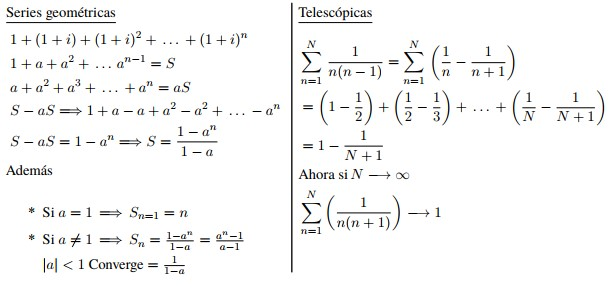
\includegraphics{images/3.jpg}

\begin{remark}
\begin{align*}
&\int v^t \, dt = 1 \cdot \int v^t \, dt = \frac{\log (v)}{\log (v)}\int v^t \, dt & u = v^t \quad du = v^t \log(v)\\
&\Longrightarrow \frac{1}{\log (v)}\int v^t\log(v) \, dt =\frac{v^t}{\log(v)} + C & \Longrightarrow \int du = \int v^t \log(u) = v^t
\end{align*}

En general:
\begin{align*}
& \int u'\cdot e^{u}\, du = e^{u} + C \\
& \int u'a^{u} \, du = \frac{a^{u}}{\log(a)} + C 
\end{align*}
\end{remark}

\hypertarget{ejercicios-interuxe9s-simple}{%
\subsection{Ejercicios (interés simple)}\label{ejercicios-interuxe9s-simple}}

\begin{enumerate}
\def\labelenumi{\arabic{enumi}.}
\tightlist
\item
  ¿Cuánto interés se gana en el cuarto año si se invierten \(\$ 3000\) bajo interés simple a una tasa anual del \(5\%\) ¿Cuál es el saldo al final del cuarto año?
\end{enumerate}

Saldo final:

\(A(t) = 3,000(1+0.05(4)) = \underline{3,600}\)

\begin{enumerate}
\def\labelenumi{\arabic{enumi}.}
\setcounter{enumi}{1}
\tightlist
\item
  ¿En cuántos años se acumularán \(\$500\) a \(\$800\) con un interés del \(6\%\)?
\end{enumerate}

\(A(1) = 500, \: A(t) = 800, \: i = 6\% \\ A(t) = 500 (1 + 0.06(t)) = 800\\ \frac{800}{500} = 1+ 0.06 (t) \: \Longrightarrow \: \frac{8}{5}-1 = 0.06(t) \: \Longrightarrow \: \frac{\frac{8}{5}-1}{0.06} = t \quad \therefore\underline{\: t = 10 \, \text{años}}\)

\begin{enumerate}
\def\labelenumi{\arabic{enumi}.}
\setcounter{enumi}{2}
\tightlist
\item
  Encuentre la tasa de interés simple anual para que \(\$ 1,000\) invertido a tiempo \(t = 0\) crezca a \(\$1,700\) en 8 años.
\end{enumerate}

\(A(0) = 1,000, \: A(8) = 1,700, \: t=8 \, \text{años}\\A(8) = 1,000(1+i(8)) = 1,700 \: \Longrightarrow \: \frac{1,700}{1,000} = (1+i(8))\\ \Longrightarrow \: \frac{(1.7-1)}{8} = i = 0.087\\ \therefore \: \underline{\text{La tasa anual debe ser de } 8.7\%}\)

\begin{enumerate}
\def\labelenumi{\arabic{enumi}.}
\setcounter{enumi}{3}
\tightlist
\item
  A una tasa de interés simple, \(\$ 1,200\) invertidos en el tiempo \(t = 0\) acumula \(\$1,320\) en \(t\) años. Encuentre el valor acumulado de \(\$500\) invertido a la misma tasa de interés simple y a \(t = 0\), pero esta vez para \(2t\)
\end{enumerate}

\(A(0) = 1,200, \: A(t) = 1,320\)

\begin{enumerate}
\def\labelenumi{\alph{enumi})}
\item
  \(A(t) = 1200(1+it) = 1320 \: \Longrightarrow \: t = \frac{\frac{1320}{1200}-1}{i}\)
\item
  \(A(2t) = 500(1+i2t)\\ 500\left( 1+\underline{i}2\left( \frac{\frac{1320}{1200}-1}{\underline{i}}\right) \right) = 500 \left( 1 + 2 \left( \frac{1320}{1200} -1\right) \right) = \underline{600\, \text{acum}}\)
\end{enumerate}

\hypertarget{ejercicios-interuxe9s-compuesto}{%
\subsection{Ejercicios (interés compuesto)}\label{ejercicios-interuxe9s-compuesto}}

\begin{enumerate}
\def\labelenumi{\arabic{enumi}.}
\tightlist
\item
  Alice invierte \(\$2,200\), Su inversión crece de acuerdo al interés compuesto con una tasa de interés anual de \(4\%\) por \(t\) años en el cual acumuló \(\$8,000\). Encuentre \(t\).
\end{enumerate}

\(A(0) = 2,200,\: i=4\%,\: A(t) = \$ 8,000 \\ A(t) = 2,200(1+0.04)^t = 8,000 \: \Longrightarrow \: (1+0.04)^t = \frac{8,000}{2,200} \\ \Longrightarrow \: t\ln(1+0.04) = \ln\left( \frac{8,000}{2,200}\right) \\ \Longrightarrow t =\frac{\ln\left(\frac{8,000}{2,200} \right) }{\ln(1.04)} \\ \therefore \: \underline{t=32.91}\)

\begin{enumerate}
\def\labelenumi{\arabic{enumi}.}
\setcounter{enumi}{1}
\tightlist
\item
  Eliot recibe la herencia de su tía Ruth, cuando ella murió en su cumpleaños número 5. En su cumpleaños 18, la herencia creció a \(\$ 32,168\). Si el dinero ha estado creciendo a una tasa de interés compuesto anual de \(6.2\%\) encuentre la cantidad que le heredó la tía Ruth a Eliot.
\end{enumerate}

\(A(0) = M,\: i = 6.2\%,\: A(13) = 32,168\\ A(0) = M(1.062)^{13} = 32,168 \: \Longrightarrow \: M\frac{32,168}{(1.062)^{13}} = \underline{14,716.52}\)

\begin{enumerate}
\def\labelenumi{\arabic{enumi}.}
\setcounter{enumi}{2}
\tightlist
\item
  ¿Cuánto interés se gana en el cuarto año de una inversión de \(\$1,000\) invertida a una tasa compuesta anual efectiva de \(5\%\) ?
\end{enumerate}

\(t = 4\, \text{años}, \: M=1,000,\: i = 5\% \\ A(4) = 1,000(1+0.05)^4 = 1,215.5 \: \Longrightarrow \: 1,215.5 - 1,000 = 215.5\\ \therefore \: \underline{\text{El interés ganado es} \, \$ 215.5}\)

\begin{enumerate}
\def\labelenumi{\arabic{enumi}.}
\setcounter{enumi}{3}
\item
  A una cierta tasa de interés compuesta, el dinero se duplicará en \(\alpha\) años, se triplicará en \(\beta\) años y se multiplicará por 10 en \(\gamma\) años. Al mismo tiempo con una tasa de interés compuesta, \(\$5\) incrementa a \(\$12\) en \(n\) años. Encuentre el interés \(a\), \(b\), \(c\) tal que \(n=a\alpha + b\beta + c\gamma\)
  \begin{align*}
  & A(\alpha) = M(1 + i)^{\alpha} = 2M  & \hfill \hfill \\
  & A(\beta) = M(1+i)^{\beta} = 3M  & \textbf{Tarea} \, A(n) = 5 (1+i)^n = 12 \\
  & A(\gamma) = M(1+i)^{\gamma} = 10M
  \end{align*}
\item
  Eduardo depositó \(\$ 826\) en una cuenta de ahorros que genera intereses a una tasa de incremento del banco. Durante los primeros \(3\) años del depósito la tasa de interés anual es del \(2.6\%\). Para los próximos \(2\) años la tasa efectiva anual es del \(4.5\%\) y los siguientes \(5\) años la tasa de interés efectiva anual es del \(6\%\), ¿Cuál es el acumulado al final de \(10\) años?
\end{enumerate}

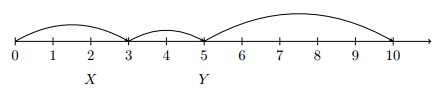
\includegraphics{images/4.jpg}

\begin{align*}
A(10) &= 826 (1+i)^{10} \\
      &= 826 (1+0.026)^3(1+0.04)^2(1+0.06)^5 = \underline{1,303.71}\\
\hfill \text{ó} \\
A(3) &= 826(1+0.026)^3=X\\
A(5) &=X(1+0.04)^2 = Y\\
\therefore \: A(10) &=Y(1+0.06)^5
\end{align*}

\hypertarget{clase}{%
\section{Clase}\label{clase}}

\textbf{Resumen}

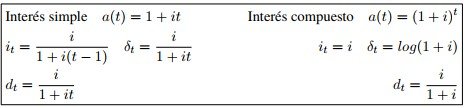
\includegraphics{images/5.jpg}

\begin{example}

\(a(t) = (1-d)^{-t}\), \(t\geq 0\), \(d\in (0,1)\)

¿Es función de acumulación?

\begin{enumerate}
\def\labelenumi{\roman{enumi})}
\item
  \(a(0) = (1-d)^{-0} = 1\)
\item
  \(a(\cdot)\) continua
\item
  \(a'(t) = \left( (1-d)^{-t}\right)' = \left( e^{-tlog(1-d)}\right)' = e^{-tlog(1-d)}(-1)log(1-d) \\ = \underbrace{-(1-d)^{-t}}_{\geq 0} \underbrace{log(1-d)}_{\geq 0} \geq 0\)
\end{enumerate}

\end{example}

\begin{itemize}
\tightlist
\item
  \(i_t\)
\end{itemize}

\begin{align*}
i_t &= \frac{a(t)-a(t-1)}{a(t-1)} = \frac{(1-d)^{-t}-(1-d)^{-(t-1)}}{(1-d)^{-(t-1)}} = \frac{(1-d)^{-(t-1)}}{(1-d)^{-(t-1)}}\left[(1-d)^{-1} - 1 \right] \\
&= \frac{1}{1-d}-1 = \frac{1-(1-d)}{1-d} = \boxed{\frac{d}{1-d} \, \text{cte.}}
\end{align*}

\begin{itemize}
\tightlist
\item
  \(d_t\)
\end{itemize}

\begin{align*}
d_t &=  \frac{a(t) - a(t-1)}{a(t)} = \frac{(1-d)^{-t} - (1-d)^{-(t-1)}}{(1-d)^{-t}} = 1-(1-d) = \boxed{d \, \text{cte.}}
\end{align*}

\begin{itemize}
\tightlist
\item
  \(\delta_t\)
\end{itemize}

\begin{align*}
\delta_t &= \frac{a'(t)}{a(t)} = \frac{\partial}{\partial t} log(a(t)) = \frac{\partial}{\partial t} log\left( (1-d)^{-t}\right) = \frac{\partial}{\partial t} (-t\cdot log(1-d))\\
& = \boxed{-log(1-d)  \, \text{cte.}}
\end{align*}

A \(\boxed{a(t) = (1-d)^t}\) se le conoce como \textbf{{modelo de descuento compuesto}}, y a \textbf{\(d\)} se le conoce como \textbf{{tasa efectiva de descuento.}}

\begin{example}

\(a(t) = \frac{1}{1-td}\), \(t\in \left[0, \frac{1}{d} \right)\), \(d\in (0,1)\)

¿Es función de acumulación?

\begin{enumerate}
\def\labelenumi{\roman{enumi})}
\item
  \(a(0) = \frac{1}{1-0d} = \frac{1}{1} = 1\)
\item
  Es continua
\item
  \(\frac{\partial}{\partial t} a(t) = \frac{\partial}{\partial t} (1 - td)^{-1} = (-1)(1-td)^{-2}(-d) = \frac{d}{(1-td)^2} > 0\), \(a(\cdot)\) es creciente.
\end{enumerate}

\end{example}

\(\textbf{Tarea:} \, i_t, \, d_t, \, \delta_t\)

A \(\boxed{a(t) = 1/(1-td)}\), \(t\in \left[0,1/d \right)\) se le conoce como \textbf{{modelo de descuento simple}} y a \(\underline{d}\) se le conoce como {tasa efectiva de descuento simple}.

\hypertarget{ejercicios-de-clase}{%
\subsection{Ejercicios de Clase}\label{ejercicios-de-clase}}

\begin{enumerate}
\def\labelenumi{\arabic{enumi}.}
\tightlist
\item
  Se requiere conocer el monto (valor acumulado) de \(\$2,770\) colocados a las tasas de interés simple que se indican a continuación:
\end{enumerate}

\begin{itemize}
\tightlist
\item
  \(17.65 \%\) anual, después de cinco años y ocho meses.
\item
  \(0.14 \%\) diario, después de un mes y medio.
\item
  \(4.85 \%\) trimestral, después de diez meses.
\end{itemize}

\textbf{La tasa manda}

\begin{enumerate}
\def\labelenumi{\alph{enumi})}
\tightlist
\item
  \(A_k(t) = k\cdot a(t)\)
\end{enumerate}

\(A_{2770}(t) = 2770(1+0.1765t)\) donde \(t\) se mide en \textbf{años}

\(A_{2770}(\text{5 años, 8 meses}) = A_{2770}\left(5+\frac{9}{12} \right)=A_{2770}\left( 5 + \frac{2}{3}\right)\)

\(= A_{2770}\left( \frac{17}{3}\right) = \underline{2770 \left( 1+0.1765\left( \frac{17}{3}\right) \right)}\)

\begin{enumerate}
\def\labelenumi{\alph{enumi})}
\setcounter{enumi}{1}
\tightlist
\item
  \(A_{2770}(t) = 2770(1+0.0014t)\), \(t\) se mide en días.
\end{enumerate}

\(A_{2770} (\text{1 mes y medio}) = A_{2770}(\text{45 días}) = \underline{2770(1+0.0014(45))}\)

\begin{enumerate}
\def\labelenumi{\alph{enumi})}
\setcounter{enumi}{2}
\tightlist
\item
  \(A_{2770}(t)=2770(1+0.0485t)\), \(t\) se mide en trimestres
\end{enumerate}

\(A_{2770}(\text{10 meses}) = A\left(3t +\frac{1}{3} \text{trimestres}\right)\)

\(A_{2770}\left(\frac{10}{3} \right) = \underline{2770\left( 1+0.0485\left(\frac{10}{3} \right) \right)}\)

\begin{enumerate}
\def\labelenumi{\arabic{enumi}.}
\setcounter{enumi}{1}
\tightlist
\item
  Calcule el monto de \(\$1,500\) al \(3\%\) de interés simple efectivo mensual después de los tiempos que se indican:
\end{enumerate}

\begin{itemize}
\item
  15 días
\item
  Seis meses
\item
  Un año y medio
\item
  Tres años
\item
  Un siglo
\item
  \(A_{1500}(t)=1500(1+0.03t)\), \(t\) se mide en \textbf{meses}
\item
  \(A_{1500}(\text{15 días}) = A_{1500}\left( \frac{1}{2} \, \text{mes}\right)= \underline{1500\left(1+0.03\left( \frac{1}{2}\right) \right)}\)
\item
  \(A_{1500}(\text{1 siglo}) = A_{1500}\left(\underset{\text{día}}{100} \cdot \underset{\text{mes}}{12}\right)=A_{1500}(1200) = \underline{1500(1+0.03(1200))}\)
\end{itemize}

\begin{enumerate}
\def\labelenumi{\arabic{enumi}.}
\setcounter{enumi}{2}
\tightlist
\item
  Dados los siguientes capitales (iniciales), montos y plazos, calcule la tasa de interés simple efectiva anual correspondiente:
\end{enumerate}

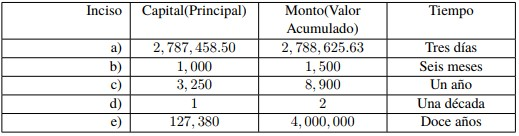
\includegraphics{images/6.jpg}

\begin{enumerate}
\def\labelenumi{\alph{enumi})}
\tightlist
\item
  \(M = 2,787,458.50\)
\end{enumerate}

\(2787458.50\left( 1+\underbrace{i}_{i\,\text{ anual}} \cdot \frac{3}{365}\right) = 2788625.63\). Despejar \(i \: \ldots\)

\begin{enumerate}
\def\labelenumi{\alph{enumi}.}
\setcounter{enumi}{3}
\tightlist
\item
  \(1(1+i\cdot 10) = 2\). Despejar \(i\: \ldots\)
\end{enumerate}

\begin{enumerate}
\def\labelenumi{\arabic{enumi}.}
\setcounter{enumi}{10}
\tightlist
\item
  Un inversionista se encuentra ante la opción de elegir una de las siguientes alternativas:
\end{enumerate}

\begin{itemize}
\tightlist
\item
  Compra hoy una bodega en \(\$20,500,000\), con la posibilidad de venderla en \(\$40,500,000\) dentro de dos años y medio.
\item
  Prestar dicho dinero a una tasa del \(2.3\%\) mensual simple.
\end{itemize}

¿Qué le recomendaría usted al inversionista?

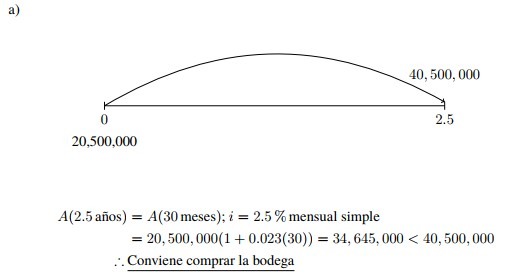
\includegraphics{images/7.jpg}

\begin{itemize}
\tightlist
\item
  Si nos dan \(a(t)\) ¿podrían obtener \(\delta_t\)? \textbf{Sí}
\end{itemize}

Mediante la definición.

\begin{align*}
&\delta_t = \frac{a'(t)}{a(t)} = \frac{\partial}{\partial t} \log(a(t))&
\end{align*}

\begin{itemize}
\tightlist
\item
  Si nos dan \(\delta_t\) ¿Podrían obtener \(a(t)\)? \textbf{Sí}
\end{itemize}

\begin{align*}
&\delta_s = \frac{\partial}{\partial s} \log(a(s))&\\
& \Longrightarrow \: \int_{0}^{t} \delta_s \, ds = \int_{0}^{t} \frac{\partial}{\partial s}\log(a(s)) \, ds &\\
& \stackrel{\text{TFC}}{\Longrightarrow} \int_{0}^{t} \delta_s \, ds  = \log(a(t)) - \log(a(0)) \Longrightarrow  \int_{0}^{t} \delta_s \, ds = \log(a(t)) - \log(1)&\\
&\Longrightarrow \exp\left\lbrace  \int_{0}^{t} \delta_s \, ds \right\rbrace  = a(t) \: \ldots \: (\ddot\smile)&
\end{align*}

\begin{itemize}
\tightlist
\item
  Si nos dan \(a(t)\), ¿\(i_t\)? \textbf{Sí}
\end{itemize}

\begin{align*}
&i_n = \frac{a(n)-a(n-1)}{a(n-1)}&
\end{align*}

\begin{itemize}
\tightlist
\item
  Si nos dan \(i_n\), ¿\(a(t)\)? \underline{Sí, parcialmente}
\end{itemize}

\begin{align*}
&i_n = \frac{a(n)-a(n-1)}{a(n-1)} \: \left(i_n \cdot a(n-1) = a(n) - a(n-1) \right) &\\
&\Longrightarrow\: i_n \cdot a(n-1) + a(n-1) = a(n)&\\
&\Longrightarrow\: a(n) = \underbrace{a(n-1)}_{\text{Recursivamente}}\left[1+i_n \right] &\\
&a(n) = \stackrel{\mbox{$\downarrow$}}{a(n-2)}\left( 1+i_{n-1}\right) \left[1+i_n\right]&\\
&\text{Recursivamente}&\\
&a(n) =  \left(1 + i_1 \right) \left(1+i_2 \right) \:\cdots\: \left( 1 + i_n\right) = \prod_{k=1}^{n} \left( 1+ i_k\right)&\\
&\boxed{\therefore \: a(n) = \prod_{k=1}^{n} \left( 1+ i_k\right)}&
\end{align*}

\begin{itemize}
\tightlist
\item
  Si nos dan \(a(t)\), ¿\(d_n\)? \textbf{Sí}
\end{itemize}

\begin{align*}
&d_n = \frac{a(n)-a(n-1)}{a(n)}&
\end{align*}

\begin{itemize}
\tightlist
\item
  \(d_n\), ¿\(a(t)\)? \textbf{Sí, parcialmente} \(\quad\) \textbf{{Tarea}}
\end{itemize}

\begin{example}
Considere la función \(\left( 1 + \frac{i^{(m)}}{m}\right)^{mt}, \: m\in \mathbb{N}_+, \: i^{(m)}>0\)
\end{example}

\textbf{Nota:} \(i^{m}\) es notación, no exponenciación.

¿Es \(a(\cdot)\) función de acumulación?

\begin{enumerate}
\def\labelenumi{\roman{enumi})}
\item
  \(a(0)=\left( 1 + \frac{i^{(m)}}{m}\right)^{m\cdot 0} = 1\)
\item
  , \(\:\) iii)
\end{enumerate}

\(a(t) =\left[ \left( 1 +\frac{i^{(m)}}{m}\right)^{m}\right]^t\) es una función del tipo exponencial, por tanto es continua, y como \(\left( 1 +\frac{i^{(m)}}{m}\right)^{m} > 0\), también es creciente.

A \(\boxed{\left( 1 + \frac{i^{(m)}}{m}\right)^{mt}}\) se le conoce como \textbf{{modelo de interés nominal convertible m veces.}}

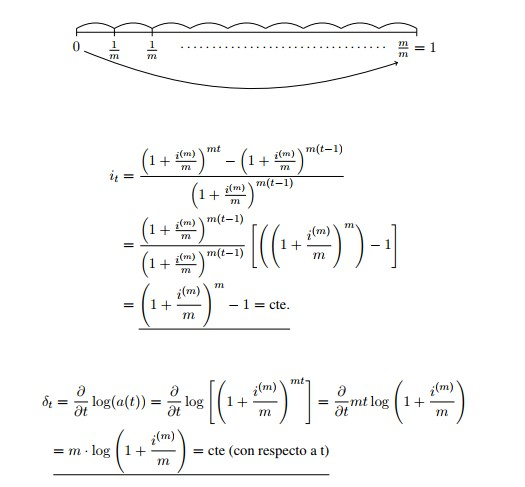
\includegraphics{images/8.jpg}

A \(\underline{i^{(m)}}\) se le conoce como \textbf{{de interés por periodo capitalizable m veces por periodo}} o \textbf{{tasa de interés por periodo convertible veces por periodo}} y establece que el interés que se nos paga por \(\underline{m-\text{ésimo}}\) de periodo es \(\frac{i^{(m)}}{m}\).

.

\begin{enumerate}
\def\labelenumi{\arabic{enumi}.}
\item
  Si el periodo es anual e \(i^{(3)} = 10\%\) significa que nos paga \(\frac{10\%}{3}\) cada \textbf{tercio de año}, i.e, se nos paga \(3.33\%\) cada \textbf{cuatrimestre}.
\item
  Si el periodo es anual e \(i^{(4)} = 10\%\) significa que se nos pagó \(\frac{10\%}{4}\) cada \textbf{cuarto de año}, i.e, se nos paga \(2.5\%\) cada \textbf{trimestre}.
\item
  Si el periodo es anual e \(i^{(12)} = 10\%\) significa que \(\ldots\; \frac{10\%}{12}\) cada \textbf{doceavo de año}, \(\ldots \: \frac{10\%}{12}\) cada \textbf{mes}.
\item
  \(\ldots\) es \textbf{semestral} e \(i^{(3)} = 10\% \: \ldots \: \frac{10\%}{3}\) cada \textbf{tercio de semestres}, i.e, \(\ldots \: 3.33\%\) cada \textbf{bimestre}.
\item
  \(\ldots\) bianual e \(i^{(2)} = 10\% \: \ldots \: \frac{10\%}{2}\) cada \textbf{mitad de bi-año}, \(\ldots \: 5\%\) cada \textbf{año}.
\item
  \(\ldots\) es quinquenal e \(i^{(2)} = 30\% \: \ldots \: \frac{30\%}{60}\) cada \textbf{sesentavo de quinquenio} \(0.5\%\) cada \textbf{mes}.
\item
  \(\ldots \:\) \textbf{anual} e \(i^{(365)} = 5\% \: \ldots \: \frac{5\%}{365}\) cada \(\underline{365-\text{avo}}\) de año\}, \(\ldots\:, \frac{5\%}{365}\) cada \textbf{día}.
\end{enumerate}

\begin{remark}
Si se da una \(i^{(m)}\) y \textbf{no} se especifica el periodo se supone \textbf{anual}.
\end{remark}

\hypertarget{ejercicios}{%
\subsection{Ejercicios}\label{ejercicios}}

\begin{enumerate}
\def\labelenumi{\arabic{enumi}.}
\setcounter{enumi}{11}
\tightlist
\item
  Daniel decide prestarle \(\$2,000,000\) a su amiga Adriana (él es un acaudalado ayudante de profesor). Adriana le pagará \(\$3,600,000\) dentro de tres años. ¿Qué tasa de interés simple semestral debería ofrecer un banco para que Daniel no le prestara el dinero a Adriana y mejor decidiera invertirlo de dicho banco (y convertirse en el peor de los amigos)?
\end{enumerate}

\begin{align*}
&a(t) =1+it&\\
&3,600,000 = 2,000,000(1 + i\cdot \stackrel{\stackrel{3\, \text{años} = 6\, \text{semestres}}{\uparrow}}{6}) \Longrightarrow i = \frac{\frac{36}{10}-1}{6} = 13.33^{-}\%&
\end{align*}

Si un banco le ofrece una tasa de interés simple semestral mayor que \(13.33^{-} \%\), Daniel preferirá invertir en el banco.

\(= \, :\) le da igual.

\(< \, :\) a la amiga.

\begin{enumerate}
\def\labelenumi{\arabic{enumi}.}
\setcounter{enumi}{8}
\tightlist
\item
  Encontrar la tasa de interés mensual simple que se obtiene cuando se invierten \(\$210,000\) y al cabo de diez meses se puede retirar \(\$311,650\).
\end{enumerate}

\begin{align*}
&210,000(1+i\cdot 10) = 311,650& \\
&i \frac{\frac{311,650}{210,000}-1}{10} = \underline{4.84\% \, \text{mensual }}&
\end{align*}

Considere la función \(\boxed{\color{black}a(t) = \left(1 - \frac{d^{(p)}}{p}\right)^{-pt}} \color{black}, \: d^{(p)} \in (0,1)\).

¿\(a(t)\) es función de acumulación?

\begin{enumerate}
\def\labelenumi{\roman{enumi})}
\item
  \(a(0) = \left( 1 - \frac{d^{(p)}}{p}\right)^{-p\cdot0} = 1\)
\item
  , iii) \(a(t) = \left( \left(1 - \frac{d^{(p)}}{p}\right)^{-p}\right)^{t}\) es de tipo exponencial, por lo tanto es continua y es creciente pues \(\left(1 - \frac{d^{(p)}}{p}\right)^{-p} > 0\).
\end{enumerate}

\(\therefore \: a(t) = \left(1 - \frac{d^{(p)}}{p}\right)^{-pt}\) es función de acumulación.

\begin{align*}
\cdot \, i_t &= \frac{\left(1 - \frac{d^{(p)}}{p}\right)^{-pt} - \left(1 - \frac{d^{(p)}}{p}\right)^{-p(t-1)}}{\left(1 - \frac{d^{(p)}}{p}\right)^{-p(t-1)}} = \frac{\left(1 - \frac{d^{(p)}}{p}\right)^{-p(t-1)}}{\left(1 - \frac{d^{(p)}}{p}\right)^{-p(t-1)}} \left[ \left(1 - \frac{d^{(p)}}{p}^{-p}\right) -1\right] \\
&= \underline{\left(1 - \frac{d^{(p)}}{p}\right)^{-p} -1 , \, \text{es cte con respecto a t.}} \\
\cdot \, d_t &= \frac{a(t)-a(t-1)}{a(t)} = 1 - \frac{a(t-1)}{a(t)} = 1- \frac{\left(1 - \frac{d^{(p)}}{p}\right)^{-p(t-1)}}{\left(1 - \frac{d^{(p)}}{p}\right)^{-pt}}\\
&= \underline{1-\left(1 - \frac{d^{(p)}}{p}\right)^{p}\, \text{es constante con respecto a t.}}\\
\cdot \, \delta_t &= \frac{\partial}{\partial t} \log(a(t)) = \frac{\partial}{\partial t}\log\left[\left(1 - \frac{d^{(p)}}{p}\right)^{-pt} \right] = \frac{\partial}{\partial t} \left( -pt\cdot\log\left(1 - \frac{d^{(p)}}{p}\right)\right)\\
&= \underline{-p\log\left(1 - \frac{d^{(p)}}{p}\right) \, \text{es constante con respecto a t.}} 
\end{align*}

A \textbf{{\(d^{(p)}\)}} se le conoce como {``tasa de descuento por periodo convertible \(p\) veces por periodo''} ó {``tasa de descuento nominal por periodo capitalizable \(p\) veces por periodo''}.

Dadas 2 funciones de acumulación \(a_1(\cdot)\) y \(a_2(\cdot)\) {son equivalentes al tiempo \(t^{*}\)} si {\(a_1(t^{*})= a_2(t^{*})\)}, y se denota como {\(a_1 \underset{t^{*}}{\sim }a_2\)}.

Dadas 2 funciones de acumulación \(a_1(\cdot)\) y \(a_2(\cdot)\) se dice que \(a_1(\cdot)\) y \(a_2(\cdot)\) {son equivalentes} si \(\forall \: t\in[0,\infty) \: a_1(t) = a_2(t)\) y se denota como {\(a_1 \sim a_2\)}

Claramente si \(a_1 \sim a_2\), entonces \(a_1 \underset{t}{\sim} a_2\) para cualquier \(t \in [0, \infty)\)

¿\(a_1\underset{t^{*}}{\sim} a_2\:\Longrightarrow \: a_1\sim a_2\)?

\(\underline{\text{No necesariamente}}\), contraejemplo: dibujo \(\searrow\)

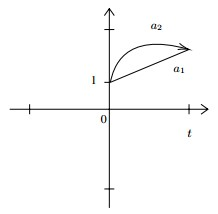
\includegraphics{images/9.jpg}

\begin{proposition}
Sean \(a_1, \, a_2\) funciones de acumulación, si

\begin{enumerate}
\def\labelenumi{\arabic{enumi})}
\item
  \(a_1 \underset{t^{*}}{\sim} a_2\) para algún \(t^{*} \in [0, \infty)\)
\item
  \(a_1\) y \(a_2\) tienen fuerza de interés constante,
\end{enumerate}

entonces \(a_1 \sim a_2\)
\end{proposition}

\begin{proof}
Sean \(\delta_{1,t}\) y \(\delta_{2,t}\) las fuerzas de interés de las funciones \(a_1(\cdot)\) y \(a_2(\cdot)\) respectivamente.

Por una observación que hicimos ayer

\begin{align*}
a_1(t) &= e^{\int_{0}^{t} \delta_{1,s} \, ds} & a_2(t) &= e^{\int_{0}^{t} \delta_{2,s} \, ds}\\
&= e^{\int_{0}^{t} \delta^{(1)} \, ds}   &&= e^{\int_{0}^{t} \delta^{(2)} \, ds}\\
&= e^{\delta^{(1)}\cdot t}   &&= e^{\delta^{(2)}\cdot t}
\end{align*}
pues \(\delta_{1,t} = \delta^{(1)}\) cte y \(\delta_{2,t} = \delta^{(2)}\) cte.

pero por (1) \(a_1(t^{*}) = a_2(t^{*})\) entonces \(e^{\delta^{(1)}t^{*}} = e^{\delta^{(2)}t^{*}}\: \Longrightarrow \: \left( e^{\delta^{(1)}}\right) ^{t^*} = \left( e^{\delta^{(2)}}\right) ^{t^*} \\ \Longrightarrow \: e^{\delta^{(1)}} = e^{\delta^{(2)}}\: \ldots \: (*)\)

Entonces para cualquier \(t\in [0,\infty) \quad a_1(t) = e^{\delta^{(1)}t} \stackrel{\mbox{(*)}}{=} e^{\delta^{(2)}t} = a_2(t)\)
\[\: \therefore a_1(t) = a_2(t)\]
\[\: \therefore a_1 \sim a_2\]
\end{proof}

{Tarea:}

{1. Demostrar que \(a_1 \sim a_2\) es relación de equivalencia}

{2. Demostrar que \(a_1 \underset{t^{*}}{\sim} a_2\) es relación de equivalencia}

Esta proposición nos pide que las funciones de acumulación tengan fuerza de interés constante.

Ya vimos muchas funciones de acumulación con fuerza de interés constante.

\(\hspace{1.3cm} a(t) \hspace{3cm} \delta_t\)

\begin{enumerate}
\def\labelenumi{\arabic{enumi}.}
\item
  \((1+i)^t \hspace{1cm} \longrightarrow \; \log(1+i)\)
\item
  \((1-d)^{-t} \hspace{0.7cm} \longrightarrow \; -\log(1-d)\)
\item
  \(\left(1-\frac{d^{(p)}}{p} \right)^{-pt} \longrightarrow \; -p\log\left(1 - \frac{d^{(p)}}{p}\right)\)
\item
  \(\left(1 + \frac{i^{(m)}}{m} \right)^{mt} \: \longrightarrow \; m\log\left(1 + \frac{i^{(m)}}{m} \right)\)
\end{enumerate}

Según la proposición, 1., 2., 3. y 4. son equivalentes y se escribe:

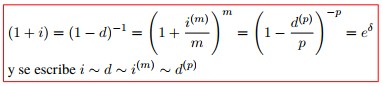
\includegraphics{images/10.jpg}

Esto significa que por ejemplo si \(i\sim d^{(p)}\), entonces \((1+i) = \left( 1 - \frac{d^{(p)}}{p}\right)^{-p}\) ó también \(i\sim d\) entonces \((1+i) = (1-d)^{-1}\) ó también \(i^{(m)} \sim d^{(p)}\) entonces \(\left(1+\frac{i^{(m)}}{m} \right)^m = \left( 1 - \frac{d^{(p)}}{p}\right)^{-p}\).

\textbf{Importante:} cuando se hable de tasas de interés \(i\) se supone el \textbf{modelo compuesto}.

\hypertarget{ayudantuxeda-1}{%
\section{Ayudantía}\label{ayudantuxeda-1}}

\textbf{De la tarea}

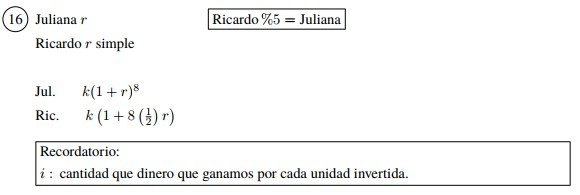
\includegraphics{images/11.jpg}
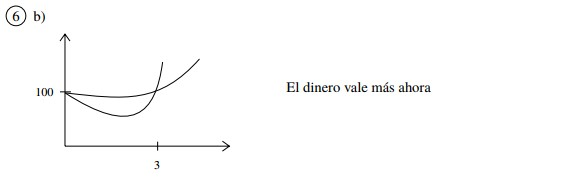
\includegraphics{images/12.jpg}
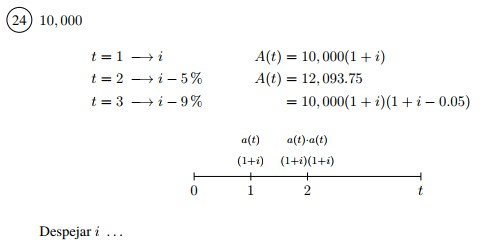
\includegraphics{images/13.jpg}

\hypertarget{clase-1}{%
\section{Clase}\label{clase-1}}

\begin{enumerate}
\def\labelenumi{\arabic{enumi}.}
\item
  \(a_1 \underset{t^{*}}{\sim} 1_2 \: \longrightarrow \: a_1(t^{*}) = a_2(t^{*})\)
\item
  \(a_1 \sim a_2 \: \longrightarrow \: \forall \, t \; a_1(t) = a_2(t)\)
\item
  \(\sim \: \Longrightarrow \: \underset{t^{*}}{\sim} \quad \forall\, t^{*}\)
\item
  \(\underset{t^{*}}{\sim} \: \nRightarrow \: \sim\)
\item
  \(\delta_t^{(1)}=\delta^{(1)}\, ; \, \delta_t^{(2)} = \delta^{(2)} \: \longrightarrow \: \underset{t^{*}}{\sim} \, \Longrightarrow \, \sim\)
\end{enumerate}

\textbf{OJO:} \(\underline{i \sim d \:\nRightarrow \: i \neq d}\)

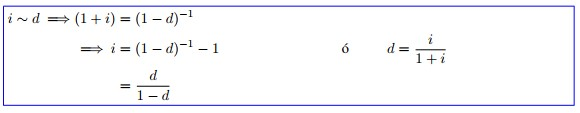
\includegraphics{images/14.jpg}

De hecho

\begin{proposition}

Si \(i \sim d \sim \delta \sim d^{(p)} \sim i^{(m)}\) entonces

\begin{enumerate}
\def\labelenumi{\arabic{enumi})}
\item
  \(\lim_{m \to \infty} i^{(m)} = \delta\)
\item
  \(\lim_{p \to \infty} d^{(p)} = \delta\)
\item
  \(d<d^{(p)}< \ldots < d^{()}< \delta < i^{()} < \ldots < i\)
\end{enumerate}

\end{proposition}

Sea \(a(\cdot)\) una función de acumulación. Se define la correspondiente {función de descuento o función valor presente} como:
\[\boxed{V_a(t) : = \frac{1}{a(t)}}\]
\(V_a(t)\) representa la cantidad de \(\$\) que \textbf{hoy} se tendría que invertir para que al final de \(t\) periodos se tuviera \(\$1\), pues
\[V_a(t) \cdot a(t) = \frac{1}{a(t)} a(t) = 1\]

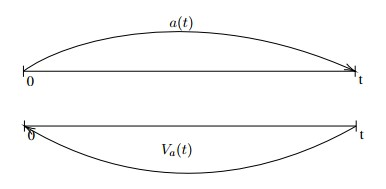
\includegraphics{images/15.jpg}

\textbf{OJO:}

Alguno libros ocupan la notación \(V_a(t) = a^{-1}(t)\)

\begin{remark}

.

\begin{enumerate}
\def\labelenumi{\arabic{enumi})}
\item
  \(V_a(0) = \frac{1}{a(0)} = \frac{1}{1} = 1\)
\item
  \(t \longmapsto V_a(t)\) es \textbf{no-decreciente} pues \(t \longmapsto a(t)\) es no-decreciente
\item
  \(V_a(\cdot)\) es también continua por pedazos.
\end{enumerate}

\end{remark}

¿Cómo me dirían qué tan buena es una función de valor presente?

Sea \(a(t)\) una función de acumulación. Se define la {fuerza de descuento de \(a(\cdot)\)} como:
\[\boxed{\color{black} \delta_{t^{*}}:= \frac{-\frac{\partial}{\partial t}V_a(t)}{V_a(t)}}\]

\begin{proposition}
Sea \(a(\cdot)\) una función de acumulación y sean \(\delta_t\) y \(\delta_{t^*}\) sus correspondientes fuerzas de interés y descuento respectivamente.
Entonces \(\delta_t = \delta_{t^{*}}\)
\end{proposition}

\begin{proof}
\begin{align*}
\delta_{t^{*}} &= \frac{-\frac{\partial}{\partial t} V_a(t)}{V_a(t)} = - \frac{\frac{\partial}{\partial t}\frac{1}{a(t)}}{\frac{1}{a(t)}} = - \frac{\frac{a(t) \cdot 0 - 1\cdot a'(t)}{\left(a(t) \right)^2 }}{\frac{1}{a(t)}} \\
& = -\frac{-a'(t)a(t)}{\left(a(t) \right)^{2}} = \frac{a'(t)}{a(t)} = \delta_t  
\end{align*}
\end{proof}

Se dice que una función de acumulación es un {modelo de descuento simple} si:

\begin{enumerate}
\def\labelenumi{(\arabic{enumi})}
\item
  \(a(\cdot)\) sea diferenciable, equivalente \(V_a(\cdot)\) sea diferenciable.
\item
  \(V_a(1) = 1-d\)
\item
  \(V_a(t+s)+1 = V_a(t) + V_a(s) \; \forall \, s,t \in [0, 1/d)\).
\end{enumerate}

\begin{proposition}
Si \(a(\cdot)\) es un \textbf{modelo de descuento simple}, entonces \(\boxed{\color{black}a(t) = \frac{1}{1-td}}\), \(t\in[0,1/d)\).
\end{proposition}

\begin{proof}
\begin{align*}
&\frac{\partial}{\partial t} V_a(t) \mathrel{\stackrel{\scriptscriptstyle \text{def. derivada}}{=}} \lim_{h \to 0} \frac{V_a(t+h) - V_a(t)}{h} \mathrel{\stackrel{\scriptscriptstyle \text{(3)}}{=}} \lim_{h \to 0} \frac{V_a(t) + V_a(h) -1 - V_a(t)}{h}\\
& = \lim_{h \to 0} \frac{V_a(h)-1}{h} = \lim_{h \to 0} \frac{V_a(h) - V_a(0)}{h} = V_a'(0)\\
& \Longrightarrow\: V_a'(s) = V'_a(0)\\
& \Longrightarrow\: \int_{0}^{t} V_a'(s) \, ds  = \int_{0}^{t} V_a'(0) \, ds\\
& \mathrel{\stackrel{\scriptscriptstyle \text{TFC}}{=}} V_a(t) - V_a(0) = V_a'(0)\cdot t \Longrightarrow\: V_a(t) = 1 + V_a'(0)\cdot t \: \ldots \: (\ddot\smile)\\
&\text{Pero por (2)} \hspace{1cm} V_a(1) = 1-d \mathrel{\stackrel{(\ddot\smile)}{=}} 1 + V_a'(0) \cdot 1\\
&\Longrightarrow V_a'(0) = -d \: \ldots \: (*)\\
&\hfill&\\
&\text{Sustituimos} \: (*)\: \text{en} \: (\ddot\smile)\\
& V_a(t) = 1-dt\\
&\Longrightarrow\: \frac{1}{a(t)} = 1 -dt\\
&\Longrightarrow\: a(t) = \frac{1}{1-td}   
\end{align*}
\end{proof}

Se dice que una función de acumulación \(a(\cdot)\) es un {modelo de descuento compuesto} si:

\begin{enumerate}
\def\labelenumi{(\arabic{enumi})}
\item
  \(a(\cdot)\) es diferenciable
\item
  \(V_a(1) = 1-d\)
\item
  \(V_a(t+s) = V_a(t)\cdot V_a(s) \; \forall \: s,t\).
\end{enumerate}

\begin{proposition}
Si \(a(\cdot)\) es un {modelo de descuento compuesto} entonces \(\boxed{\color{black}a(t) = (1-d)^{-t}}\)
\end{proposition}

\begin{proof}
{\(\boxed{\text{Tarea}}\)}
\end{proof}

\hypertarget{ayudantuxeda-2}{%
\section{Ayudantía}\label{ayudantuxeda-2}}

\textbf{Resolución de la tareita}

\begin{align*}
2 &= (1+i)^{\alpha}, \: 3 = (1+i)^{\beta}, \: 10 = (1+i)^{\gamma}, \: 5(1+i)^n = 12 &\\
& \Longrightarrow (1+i)^n = \frac{12}{5}\cdot \frac{2}{2} = \frac{24}{10} = \frac{2^3\cdot 3}{(1+i)^8} = \frac{\left( (1+i)^2 \right)^3 (1+i)^{\beta} }{(1+i)^8}&\\
& = (1+i)^{3\alpha}(1+i)^{\beta} (1+i)^{-\gamma} = (1+i)^{3\alpha + \beta -\gamma}&\\
& n = 3\alpha + \beta - \gamma = a\alpha + b \beta +c \gamma &\\
\therefore \: & \underline{a=3 \: ; b=1 \: ; c = -1}
\end{align*}

\hypertarget{ejercicios-fuerza-de-interuxe9s}{%
\subsection{Ejercicios (Fuerza de Interés)}\label{ejercicios-fuerza-de-interuxe9s}}

\begin{enumerate}
\def\labelenumi{\arabic{enumi}.}
\tightlist
\item
  Suponga que tiene una tasa de descuento simple ``\(d\)'', encuentre la fuerza de interés.
\end{enumerate}

\begin{align*}
&\delta_t = \frac{a'(t)}{a(t)}&\\
& a(t) = (1-dt)^{-1}\\
& a'(t) = -1(1-dt)^{-2}(-d)\\
& \delta_t = \frac{(1-dt)^{-2}d}{(1-dt)^{-1}} = (1-dt)^{-2+1}d = \underline{\frac{d}{(1-dt)}}
\end{align*}

\begin{enumerate}
\def\labelenumi{\arabic{enumi}.}
\setcounter{enumi}{1}
\item
  Suponga la tasa de interés compuesta ``\(i\)'' encuentre la fuerza de interés
  \begin{align*}
  &a(t) = (1+i)^t&\\
  &a'(t) = (1+i)^t\ln(1+i)&\\
  &\delta_t = \frac{(1+i)^t\ln(1+i)}{(1+i)^t} = \underline{\ln(1+i)}&
  \end{align*}
\item
  Suponga que \(a(t) = (1.07)^{t/2}(1.06)^{(t^2/3)}(1.05)^{(t^3/6)}\), encuentre \(\delta_t\).
  \begin{align*}
  a(t) &= (1.07)^{t/2}(1.06)^{t^2/3}(1.05)^{t^3/6}&\\
  \delta_t &= \frac{d}{d t} \ln(1.07)^{t/2}(1.06)^{t^2/3}(1.05)^{t^3/6} = \frac{d}{d t}\left[\frac{t}{2}\ln(1.07) + \frac{t^2}{3}\ln(1.06) + \frac{t^3}{6}\ln(1.05) \right] &\\
  &=\frac{1}{2}\ln(1.07) + \frac{2t}{3}\ln(1.06) + \frac{t^2}{2}\ln(1.05)&\\
  &=\underline{\ln\left[(1.07)^{1/2}(1.06)^{2t/3}(1.05)^{t^2/2} \right]} &
  \end{align*}
\item
  Suponga \(\delta_t = \frac{4}{1-4t}\). Encuentre su función de acumulación correspondiente.
  \begin{align*}
  a(t) &= e ^{\int_{0}^{t} \frac{4}{1-4t} \, ds}  & u = 1-4s&\\
   &\int_{0}^{t} \frac{4}{1-4s} \, ds = -\int u^{-1}\, du &du = -4ds&\\
  &= -\ln|1-4s|\big|_0^t = - \ln(1-4t) -\ln(1))&\\
  &a(t) = e^{\ln(1-4t)^{-1}} = \underline{(1-4t)^{-1}}&
  \end{align*}
\item
  Se tiene una fuerza de interés \(\delta_t = 0.05 + 0.06t\). Encuentre el valor acumulado después de 3 años si se invirtió \(\$300\) hacerlo para:
\end{enumerate}

\begin{enumerate}
\def\labelenumi{\alph{enumi})}
\item
  \(t = 0\)
\item
  \(t = 4\)
\end{enumerate}

\begin{align*}
\text{a)} \; &a(t) = e^{\int_{0}^{t} 0.05 + 0.06s \, ds}&\\
&\int_{0}^{t} 0.05 + 0.06s \, ds = 0.05(s)\big|_0^t + \frac{0.06s^2}{2}\big|_0^t &\\
&a(t) = e^{0.05 + 0.03t^2}&\\
&a(3) = e^{0.05(3) + 0.03(3)^2} = (*)&\\
&\therefore \: A(3) = 300 \cdot (*) = \underline{456.58}
\end{align*}

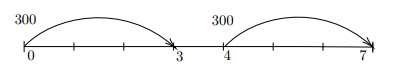
\includegraphics{images/16.jpg}

\begin{align*}
b) \; a(t) &= e ^{\int_{4}^{7} 0.05 + 0.06s} \, ds&\\
&\;\;\vdots&
\end{align*}

\begin{enumerate}
\def\labelenumi{\arabic{enumi}.}
\setcounter{enumi}{5}
\tightlist
\item
  Nos dan la siguiente fuerza de interés \(\delta_t = \frac{2t}{1+t^2}\) encuentre la función de acumulación correspondiente.
\end{enumerate}

\begin{align*}
&a(t) = e^{\int_{0}^{t} \frac{2t}{1+t^2} \, ds}& u = 1+s^2&\\
&\int_{0}^{t} \frac{25}{1+s^2} \, ds = - \int u^{-1}\, du = \ln\left(1+s^2 \right)\big|_0^t = \underline{\ln\left(1+t^2 \right) }  &du = 25ds&
\end{align*}

\begin{enumerate}
\def\labelenumi{\arabic{enumi}.}
\setcounter{enumi}{6}
\tightlist
\item
  Encuentra el valor acumulado de \(\$ 1,000\) invertido durante \(10\) años a una tasa del \(5\%\)
\end{enumerate}

\begin{align*}
&a(10) = e^{\delta_t(t)} = e^{10(0.05)}&\\
&\underline{A(10) = 1000e^{10(0.05)}}&
\end{align*}

\begin{enumerate}
\def\labelenumi{\arabic{enumi}.}
\setcounter{enumi}{7}
\tightlist
\item
  Encuentre el valor acumulado de \(\$500\) invertido durante \(4\) años a una tasa del \(2\%\)
\end{enumerate}

\(A(4) = 500e^{4(0.02)} = \underline{541.6435}\)

\begin{enumerate}
\def\labelenumi{\arabic{enumi}.}
\setcounter{enumi}{8}
\tightlist
\item
  (Mal redactado)
\end{enumerate}

\begin{align*}
&\delta_t = 0.05 + 0.01t, \; 0\leq t \leq 4&\\
&\$100(\text{son dos pagos})&
\end{align*}

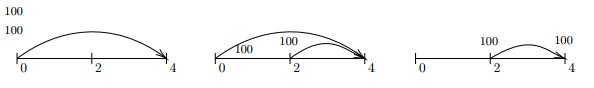
\includegraphics{images/17.jpg}

\begin{align*}
&a(t) = e^{\int_{0}^{t} \delta_s \, ds} = e^{\int_{0}^{4} 0.05+0.01s \, ds} = e^{0.05s\big|_0^4 - \frac{0.01}{2}s^2\big|_0^4}=(*)&\\
&\hfill &\\
&\text{a)} \: \Longrightarrow \: A(4) = 200(*) \, \text{si los 2 pagos en t=0}&\\
&\text{b)} \: \Longrightarrow \: A(4) = 100(*) + 100e^{\int_{2}^{4} \delta_s \, ds}&\\
&\text{c)} \: \Longrightarrow \: A(4) = 100e^{\int_{2}^{4} \delta_s \, ds} +100&
\end{align*}

\hypertarget{clase-2}{%
\section{Clase}\label{clase-2}}

\(V_a(t) = \frac{1}{a(t)} \: \longrightarrow \:\) Función valor presente.

\[\underbrace{\delta_{t^{*}}}_{ \text{Fuerza de descuento}} = \frac{-\frac{\partial}{\partial t}V_a(t)}{V_a(t)} \hspace{2cm} \delta_t^* = \underbrace{\delta_t}_{\text{Fuerza de interés}}\]

\begin{theorem}
.

\begin{align*}
&V_a(t) = 1-td&\\
&V_a(t) = (1-d)^{t}&
\end{align*}
\end{theorem}

\begin{lemma}
Para \(\alpha \in \mathbb{R} \: \lim_{m \to \infty} \left(1 + \frac{\alpha}{m} \right)^{m} = e^{\alpha}\)
\end{lemma}

\begin{proof}
\begin{align*}
&\lim_{m\to\infty} \left(1 + \frac{\alpha}{m} \right)^m =  \lim_{m\to\infty} e^{m\log\left(1 + \frac{\alpha}{m} \right)} \: \ldots \: (1)&\\
&\text{y además}&\\
&\lim_{m\to\infty}m\log\left(1 +\frac{\alpha}{m} \right) = \lim_{m\to\infty}\frac{\log\left(1 +\frac{\alpha}{m} \right)}{\frac{1}{m}} \mathrel{\stackrel{\scriptscriptstyle \text{L'Hôpital}}{=}}     \lim_{m \to \infty} \frac{\frac{1}{1+\frac{\alpha}{m}}\left(\frac{-\alpha}{m^2} \right) }{-\frac{1}{m^2}}&\\
&= \lim_{m \to \infty} \frac{\alpha}{1+\frac{\alpha}{m}} = \frac{\alpha}{1} \: \Longrightarrow \: \lim_{m\to\infty} m\log\left( 1 +\frac{\alpha}{m}\right) = \alpha &\\
&\Longrightarrow \: \exp{\left\lbrace\lim_{m\to\infty}m\log\left( 1 + \frac{\alpha}{m}\right)  \right\rbrace } = e^{\alpha} \: \Longrightarrow \: \lim_{m\to\infty}\exp{\left\lbrace m\log\left( 1 + \frac{\alpha}{m}\right)  \right\rbrace } = e^{\alpha}&\\
&(\text{pues}\, e^t \, \text{es absolutamente continua})&
\end{align*}
\end{proof}

\begin{proposition}
Si \(i^{(m)} \sim \delta\) entonces \(\lim_{m\to\infty} i^{(m)} = \delta\)
\end{proposition}

\begin{proof}
Como \(i^{(m)} \sim \delta\) entonces
\begin{align*}
&\left(1 + \frac{i^{(m)}}{m} \right)^m = e^{\delta} \: \Longrightarrow \: \lim_{m\to\infty} \left( 1 + \frac{i^{(m)}}{m}\right)^m = e^{\delta}\\
& \Longrightarrow \: e^{i^{(m)}} = e^{\delta}\\
& \therefore \: i^{(m)} \mathrel{\stackrel{\scriptscriptstyle m\rightarrow \infty}{\longrightarrow}} \delta
\end{align*}
\end{proof}

\hypertarget{anualidades}{%
\chapter{Anualidades}\label{anualidades}}

  \bibliography{book.bib,packages.bib}

\end{document}
